% Figura cuerpo B3 (4.2.3): el multiplicador en dos regímenes monetarios: el eslabón que cambia de signo
\documentclass[tikz,border=3pt]{standalone}
\usepackage[T1]{fontenc}
\usepackage[utf8]{inputenc}
\usepackage{amsmath}
\usetikzlibrary{arrows.meta,calc,positioning}
\begin{document}
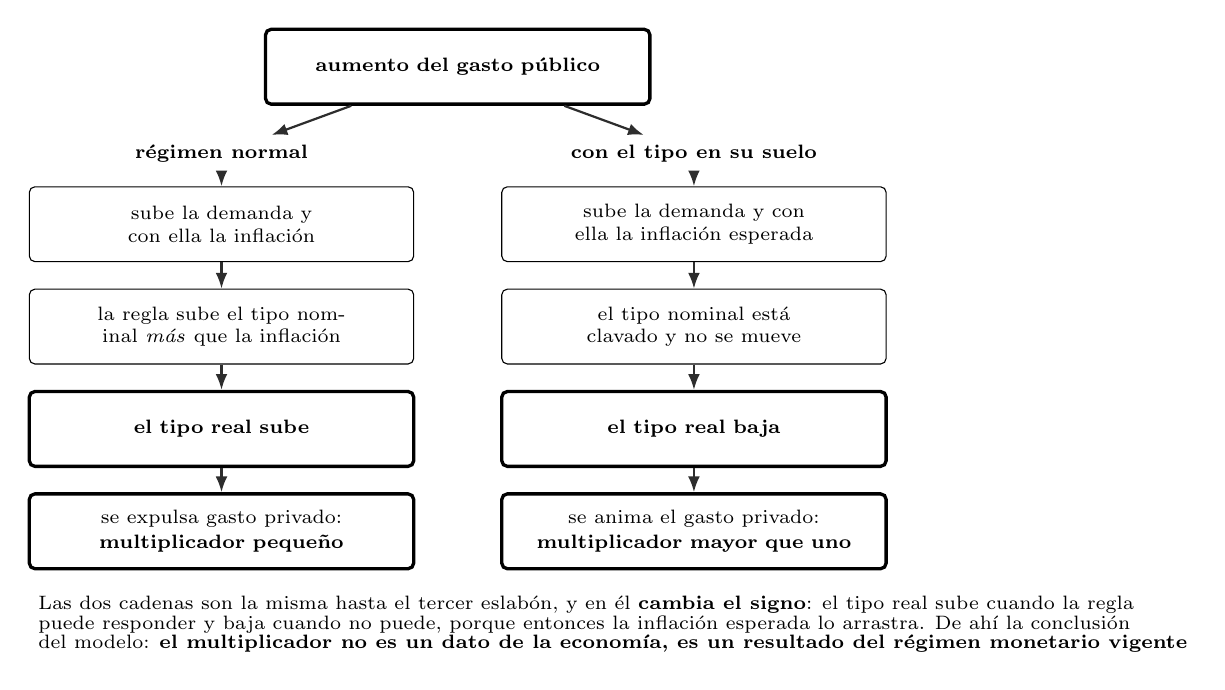
\begin{tikzpicture}[>={Latex[length=2.0mm]}, font=\scriptsize,
  caja/.style={draw, rounded corners=2pt, align=center, inner sep=4pt, text width=4.6cm, minimum height=0.95cm, font=\scriptsize},
  clave/.style={draw, very thick, rounded corners=2pt, align=center, inner sep=4pt, text width=4.6cm, minimum height=0.95cm, font=\scriptsize},
  fin/.style={draw, very thick, rounded corners=2pt, align=center, inner sep=4pt, text width=4.6cm, minimum height=0.95cm, font=\scriptsize},
  cab/.style={align=center, text width=4.6cm, font=\scriptsize\bfseries},
  fl/.style={->, thick, gray!35!black}]

  \def\cx{6.0}
  \node[clave] (G) at (0.5*\cx,6.15) {\textbf{aumento del gasto público}};

  \node[cab] (h1) at (0,5.05)    {régimen normal};
  \node[cab] (h2) at (\cx,5.05)  {con el tipo en su suelo};

  \node[caja] (a1) at (0,4.15)   {sube la demanda y con ella la inflación};
  \node[caja] (b1) at (\cx,4.15) {sube la demanda y con ella la inflación esperada};

  \node[caja] (a2) at (0,2.85)   {la regla sube el tipo nominal \textit{más} que la inflación};
  \node[caja] (b2) at (\cx,2.85) {el tipo nominal está clavado y no se mueve};

  \node[clave] (a3) at (0,1.55)   {\textbf{el tipo real sube}};
  \node[clave] (b3) at (\cx,1.55) {\textbf{el tipo real baja}};

  \node[fin] (a4) at (0,0.25)   {se expulsa gasto privado:\\[1pt]\textbf{multiplicador pequeño}};
  \node[fin] (b4) at (\cx,0.25) {se anima el gasto privado:\\[1pt]\textbf{multiplicador mayor que uno}};

  \draw[fl] (G) -- (h1);
  \draw[fl] (G) -- (h2);
  \foreach \u/\v in {a1/a2,a2/a3,a3/a4,b1/b2,b2/b3,b3/b4} \draw[fl] (\u) -- (\v);
  \draw[fl] (h1) -- (a1);
  \draw[fl] (h2) -- (b1);

  \node[align=left, anchor=north west, font=\scriptsize] at (-2.45,-0.45)
    {Las dos cadenas son la misma hasta el tercer eslabón, y en él \textbf{cambia el signo}: el tipo real sube cuando la regla\\[-1pt]puede responder y baja cuando no puede, porque entonces la inflación esperada lo arrastra. De ahí la conclusión\\[-1pt]del modelo: \textbf{el multiplicador no es un dato de la economía, es un resultado del régimen monetario vigente}};
\end{tikzpicture}
\end{document}
